\chapter{Bursts, Transients, and Multi-Messenger Quantum Astronomy}
\label{chap:e20}

\begin{chapteropening}
Up to now we have mostly looked at ``steady'' objects: the angular diameter of a star, the coherence of an accretion disk, a signal we can slowly integrate for hours. But there is another half of the universe, one that does not grant you hours, only seconds, milliseconds, even nanoseconds. A thermonuclear explosion on the surface of a white dwarf, a fireball flung out by two merging neutron stars, a radio flash sweeping across the Earth: these are ``here and gone'' events. They compress an entire chain of physical processes onto a very short time axis, forcing us to answer the same question: \textbf{when the signal is fleeting, what exactly should we record, and how do we extract physical quantities from a mere handful of photons?}

The through-line of this chapter is as follows. First we make clear why, when facing a transient, the ``event table'' of Chapter~\ref{chap:e13} (each photon carrying a time, frequency, and polarization label) is worth far more than a smooth light curve. Then we treat triggering as an act of statistical inference, not ``sound the alarm the moment you see a bright spot.'' Next we return to the book's home turf: the photon statistics and coherence of transient sources. Finally we step into the multi-messenger era, watching how the three messengers of gravitational waves, neutrinos, and photons are stitched by \textbf{time} into a single physical event. Along the way we use expanding novae, kilonovae, gamma-ray burst afterglows, and tidal disruption events as four real worked examples.
\end{chapteropening}

\section{The fast-changing universe: why we keep a time tag on every photon}
\label{sec:e20-fast}

Let us set the scene. A \textbf{light curve} is a line obtained by binning photons in time, counting the number in each bin, and connecting them. It is intuitive, but it does something irreversible: it smears a detail like ``a 512\,nm photon arrived at second 3.417\,922'' into ``the bin at second 3.4 contains 217 photons.'' For a star that slowly brightens, no harm is done; but for a transient, the temporal structure is itself the physics.

In the prompt emission of a gamma-ray burst (GRB), the light can fluctuate violently on scales of \(10^{-2}\,\mathrm{s}\); the main pulse of a fast radio burst (FRB) is often only a millisecond wide, with sub-millisecond fine structure inside it; and each pulse of a pulsar arrives with clocklike precision on a millisecond period. Once these structures are averaged away by coarse binning, they can never be recovered. This is why Chapter~\ref{chap:e13} insists on writing every photon candidate as a row in the event table, preserving its arrival time \(t\), frequency/energy channel, and polarization channel, rather than storing only a curve. This is not fastidiousness: it is because the likelihood below loses no information only when it is \textbf{unbinned}.

Denote the \textbf{instantaneous arrival rate} of photons in a given detection channel by \(\lambda(t)\), in units of \(\mathrm{s^{-1}}\). Chapter~\ref{chap:e03} explained that over an extremely short interval the probability of a photon appearing is proportional to the rate times the duration, and independent of the others; this is an \textbf{inhomogeneous Poisson point process}. Chapter~\ref{chap:e14} already derived its log-likelihood step by step, by ``slicing time into infinitely narrow cells and taking \(\Delta t\to0\)''; here we simply invoke and use that result:
\begin{equation}
  \ln L=\sum_{j=1}^{N}\ln \lambda(t_j)-\int_{t_{\rm min}}^{t_{\rm max}}\lambda(t)\,dt .
  \label{eq:e20-poisson-likelihood}
\end{equation}
\begin{formulaexplain}
\(\ln L\) is the log-likelihood of the event table under an inhomogeneous Poisson process. The first term scores the model rate at \textbf{each actual photon arrival time} \(t_j\), adding credit where a photon lands in a high-rate region; the second term subtracts the \textbf{total photon number} predicted by the model over the whole window. The two pull against each other, so a model that ``only spikes at the events'' cannot cheat.
\end{formulaexplain}
Symbol by symbol: \(N\) is the number of photons in the window \([t_{\rm min},t_{\rm max}]\) (a dimensionless count), \(\{t_j\}\) are their arrival times (in s), and \(\lambda(t)\) is the rate model (in \(\mathrm{s^{-1}}\)). The pedagogical point of this expression lies in its ``balance structure'': the first term rewards the model for placing rate where photons actually appear, while the second penalizes the model for raising the rate where there are no photons: try to bluff, and one of the two terms will dock your score.

Why insist on unbinned data? Imagine a burst that rises extremely fast; the information about \(t_0\) (the onset time) may be carried by just the earliest three to five photons. If you first bin the data into \(0.1\,\mathrm{s}\) bins, those few photons get averaged together with the rest of the bin into a single number, and the sharp information about the onset evaporates on the spot. Equation~\eqref{eq:e20-poisson-likelihood} eats the raw times \(t_j\) directly, so it can squeeze out what a binned curve cannot. This is also why the chapter repeatedly stresses ``keep the time tag in the event table.''

One of the most commonly used rate models is a ``fast-rise, slow-decay'' trigger window:
\begin{equation}
  \lambda(t)=b+A\exp\!\left[-\frac{t-t_0}{\tau}\right]H(t-t_0),
  \label{eq:e20-exponential-rate}
\end{equation}
\begin{formulaexplain}
\(\lambda(t)\) is a fast-rise, slow-decay rate model: \(b\) is the background rate, \(A\) is the excess rate at the instant of the burst, \(t_0\) is the physical onset time, \(\tau\) is the decay timescale, and \(H\) is the step function (ensuring this term is absent before \(t_0\)).
\end{formulaexplain}
Here \(b\) and \(A\) are both in \(\mathrm{s^{-1}}\), while \(t_0\), \(\tau\), and \(t\) are in s, and \(H(x)\) is the Heaviside step function (0 for \(x<0\), 1 for \(x\ge0\), dimensionless). To let the reader feel that the formula describes a real observation, let us compute the integral of its second term: over the window \(t>t_0\),
\[
  \int_{t_0}^{t_{\rm max}}\!\Big(b+Ae^{-(t-t_0)/\tau}\Big)\,dt
  = b\,(t_{\rm max}-t_0)+A\tau\Big(1-e^{-(t_{\rm max}-t_0)/\tau}\Big).
\]
When \(t_{\rm max}-t_0\gg\tau\), the exponential term goes to 0, and the total photon number contributed by the source is about \(A\tau\), that is, ``peak rate times decay timescale,'' a very intuitive quantity. The \(\tau\) of a GRB prompt can be as short as \(10^{-2}\,\mathrm{s}\), the effective decay timescale of an optical afterglow is hours to days, and the \(\tau\) of novae and tidal disruption events can be as long as tens or even hundreds of days. The same formula spans more than four orders of magnitude in timescale, which is precisely the breadth of the word ``transient.''

\section{Triggering is an act of statistical inference, not ``sound the alarm the moment you see a bright spot''}
\label{sec:e20-trigger}

Transient observation begins with a trigger, but the trigger is itself already a judgment: ``the handful of photons I see, are they a new burst, or a background fluctuation?'' To get it right, we must start from a more general rate model. For the \(k\)-th detection channel, the event rate is the background plus the instrument's response to the source flux:
\begin{equation}
  \lambda_k(t)=b_k(t)+A_{{\rm eff},k}(t)
  \int R_k(\nu,p,t)\,F_\nu(t,p)\,d\nu ,
  \label{eq:e20-rate-response}
\end{equation}
\begin{formulaexplain}
\(\lambda_k\) is the rate of the \(k\)-th channel, \(b_k\) is the background, \(A_{{\rm eff},k}\) is the effective area, \(R_k\) is the instrument response (encompassing bandwidth, quantum efficiency, polarization selection, and time response), and \(F_\nu\) is the source's photon flux at frequency \(\nu\) and polarization \(p\). The observed rate is the result of the ``source'' passing through the ``instrument'' and then having the ``background'' added on top.
\end{formulaexplain}
As for units: \(\lambda_k\) is in \(\mathrm{s^{-1}}\), \(b_k\) is in \(\mathrm{s^{-1}}\) (the sum of airglow, host galaxy, dark counts, and false triggers), \(A_{{\rm eff},k}\) is the effective area (\(\mathrm{cm^2}\)), \(R_k\) is a dimensionless response weight, and \(F_\nu\) is the photon flux per unit area per unit frequency (\(\mathrm{cm^{-2}\,s^{-1}\,Hz^{-1}}\)). The single-channel rate of an optical transient can range from less than \(1\,\mathrm{s^{-1}}\) all the way to \(10^6\,\mathrm{s^{-1}}\); high-energy detectors often record in coarser energy channels, while fast radio and optical detectors strive to push their time stamps down to sub-microsecond or even nanosecond precision. Equation~\eqref{eq:e20-rate-response} is the ``detailed instrumental version'' of the ``\(b+A\cdots\)'' in Equation~\eqref{eq:e20-exponential-rate}: only by separating the ``source'' from the ``instrument'' can one compare results across different telescopes.

The trigger must choose a side between two hypotheses: the transient model \(M_{\rm tr}\) (``there really is a burst'') and the background model \(M_{\rm bg}\) (``it is only background''). The language of estimation from Chapter~\ref{chap:e12} tells us that the right referee is the \textbf{odds ratio}:
\begin{equation}
  {\cal O}_{\rm tr,bg}
  =
  \frac{P(M_{\rm tr})}{P(M_{\rm bg})}
  \frac{L(D\mid M_{\rm tr})}{L(D\mid M_{\rm bg})},
  \label{eq:e20-trigger-odds}
\end{equation}
\begin{formulaexplain}
\({\cal O}_{\rm tr,bg}\) is the odds ratio of the transient model relative to the background model. It is a product of two pieces: on the left is the ratio of \textbf{prior rates} (how rare such a burst is to begin with), and on the right is the ratio of \textbf{data likelihoods} (which model the data resemble more).
\end{formulaexplain}
Here \(D\) is the event table or image-difference data, \(P(M)\) is the prior probability of the model (dimensionless), and \(L(D\mid M)\) is a likelihood like Equation~\eqref{eq:e20-poisson-likelihood}. This expression turns a piece of common sense into mathematics: the rarer the burst, the stronger the data must be before you dare to raise an alarm. Ignoring the prior ratio on the left is at the root of many ``false alarms flying everywhere.''

Beyond the prior, we also need a computable \textbf{false alarm probability}. If the expected background count within a time window \(\Delta t\) is \(\mu_b=b\,\Delta t\), then the probability that ``the background alone produces \(n\) or more photons'' is the tail of a Poisson distribution:
\begin{equation}
  P_{\rm FA}(N\ge n)=
  \sum_{m=n}^{\infty}\frac{\mu_b^m e^{-\mu_b}}{m!}.
  \label{eq:e20-false-alarm}
\end{equation}
\begin{formulaexplain}
\(P_{\rm FA}\) is the probability that the background alone produces \(n\) or more photons, and \(\mu_b=b\,\Delta t\) is the expected background count. Setting a trigger threshold is essentially drawing a red line across this Poisson tail probability.
\end{formulaexplain}
Let us plug in numbers to get a feel: if the background rate is \(b=1\,\mathrm{s^{-1}}\) and the window is \(\Delta t=0.1\,\mathrm{s}\), then \(\mu_b=0.1\). The probability that the background happens to throw up \(n\ge5\) photons is \(\sum_{m\ge5}0.1^m e^{-0.1}/m!\approx 8\times10^{-8}\), which sounds safe enough. But in reality you are not looking at just one window: a survey searches repeatedly over thousands of time windows, millions of sky pixels, dozens of energy channels, and dozens of templates. The true number of false triggers must be \textbf{multiplied by the number of trials} (the trials factor). If there are \(10^{10}\) effectively independent trials in one night, then that \(8\times10^{-8}\) above means about \(800\) false alarms. This is why FRB searches, gamma-ray triggers, and optical difference surveys, despite their \(\Delta t\) ranging from milliseconds to days and their backgrounds ranging from instrumental noise to variable-star contamination, all wrestle with the same ``trials factor'' ghost \citep{2013Sci...341...53T,2017ApJ...835...29Y,2020Natur.587...59B,2020Natur.587...54C,2020Natur.581..391M}.

\begin{figure}[tbp]
\centering
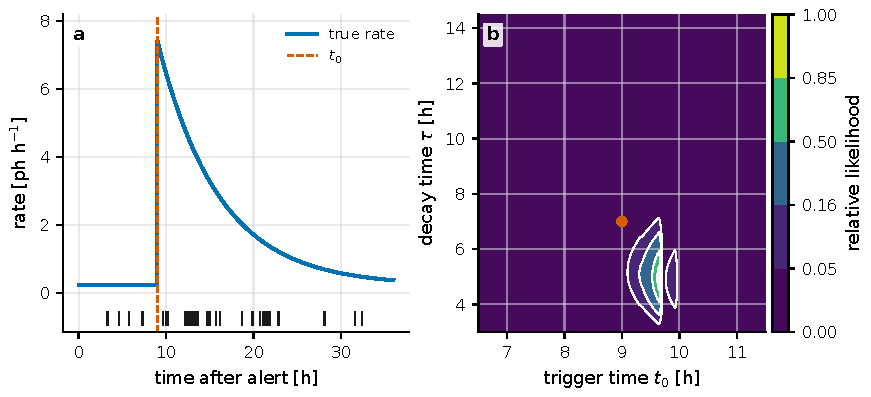
\includegraphics[width=0.92\linewidth]{figures/generated/chapter_13/ch13_transient_event_likelihood.pdf}
\caption{How an inhomogeneous Poisson event table constrains the trigger time and decay time. In the left panel each vertical line is one photon's arrival time and the blue curve is the rate model \(\lambda(t)\); the right panel writes the same event table as a relative likelihood surface over \(t_0\) and \(\tau\). A few early photons \textbf{strongly} pin down \(t_0\), while the late-time background determines whether \(\tau\) is overestimated. This is precisely the ``one reward, one penalty'' pair of terms in Equation~\eqref{eq:e20-poisson-likelihood} at work.}
\label{fig:e20-event-likelihood}
\end{figure}

\section{The photon statistics and coherence of transient sources}
\label{sec:e20-coherence}

Now back to the book's home turf: photon statistics. What kind of light does a transient source actually emit? This determines whether we can apply the coherence functions of Chapter~\ref{chap:e08} or the intensity interferometry of Chapter~\ref{chap:e10} to it.

The ``continuum face'' of the vast majority of transients is \textbf{thermal and chaotic}: the early spectra of novae, supernovae, kilonovae, and tidal disruption events can all be approximated by a blackbody photosphere (see Equation~\eqref{eq:e20-kilonova-blackbody} below). For such light, Chapter~\ref{chap:e08} gave the Siegert relation
\[
  g^{(2)}(\tau)=1+\zeta\,|g^{(1)}(\tau)|^2,
\]
that is, the photons ``pile up'' (bunch) within the coherence time. And the coherence time is set by the bandwidth; Chapter~\ref{chap:e02} gave \(\tau_c\simeq 1/\Delta\nu\). Here is an order-of-magnitude fact that is extremely real for transient observation: for a broadband optical photosphere, \(\Delta\nu\) is readily of order \(10^{13}\,\mathrm{Hz}\), so \(\tau_c\sim10^{-13}\,\mathrm{s}\), only a hundred femtoseconds. In other words, photon bunching happens on \textbf{femtosecond} scales, whereas the time bin you use to draw a light curve is a millisecond. Within a millisecond bin, the bunching has long been averaged clean, and the counting statistics degenerate into pure Poisson: the fluctuation in each bin is just the \(\sqrt N\) shot noise (Chapter~\ref{chap:e03}).

This conclusion has two faces. One is reassuring: when doing transient \textbf{photometry}, it suffices to treat the counts with Poisson errors, and the whole inference of Equation~\eqref{eq:e20-poisson-likelihood} is self-consistent. The other is a reminder: the coherence information of a thermal transient is hidden on femtosecond scales, and only \textbf{intensity interferometry} pushing time resolution to the nanosecond or even picosecond level can touch it. And the statistical precision of intensity interferometry is set by the number of \textbf{photon pairs} accumulated within the correlation window:
\begin{equation}
  N_{\rm pair}\simeq r_1 r_2\,\Delta t\,T,
  \qquad
  \delta C\simeq N_{\rm pair}^{-1/2},
  \label{eq:e20-pair-statistics}
\end{equation}
\begin{formulaexplain}
\(N_{\rm pair}\) is the number of photon pairs accumulated by two telescopes (rates \(r_1,r_2\)) within a correlation window \(\Delta t\) over a total integration time \(T\); \(\delta C\) is the correlation measurement error under pure Poisson statistics, which falls as the square root of the number of pairs.
\end{formulaexplain}
Here \(r_1,r_2\) are the event rates of the two stations (\(\mathrm{s^{-1}}\)), \(\Delta t\) is the correlation time window (s), \(T\) is the accumulated time (s), and \(N_{\rm pair}\) is dimensionless. Substituting a set of real numbers: \(r_1=r_2=10^6\,\mathrm{s^{-1}}\), \(\Delta t=100\,\mathrm{ps}=10^{-10}\,\mathrm{s}\), \(T=1\,\mathrm{h}=3600\,\mathrm{s}\), then
\[
  N_{\rm pair}\simeq (10^6)(10^6)(10^{-10})(3600)=3.6\times10^{5},
  \qquad
  \delta C\simeq (3.6\times10^5)^{-1/2}\approx1.7\times10^{-3}.
\]
That is, in one hour the correlation can be measured to the level of one part in a thousand, but note that this is only the \textbf{statistical floor}. The true error must also add on timing-synchronization error, dead time, spectral bandwidth, polarization leakage, and background fluctuations. For a fleeting source, \(T\) itself is capped by the lifetime of the burst, and this formula immediately tells you whether ``you can accumulate enough pairs before the source vanishes'', a hard constraint.

There is also a small class of transients that emit not thermal light at all but \textbf{coherent emission}: the radio pulses of FRBs and pulsars are the representatives. The criterion is the \textbf{brightness temperature} \(T_b\), the temperature that would be required ``if it were thermal radiation,'' obtained by converting the observed brightness via the Rayleigh--Jeans law. In the radio band, the photon energy is far below the thermal energy (\(h\nu\ll k_{\rm B}T_b\)), and the single-mode occupation number used in Chapters~\ref{chap:e05} and \ref{chap:e16} degenerates into a large number:
\[
  \bar n_\nu=\big[\exp(h\nu/k_{\rm B}T_b)-1\big]^{-1}
  \;\xrightarrow[h\nu\ll k_{\rm B}T_b]{}\;
  \frac{k_{\rm B}T_b}{h\nu}\gg1 .
\]
Here we have used the standard Taylor expansion \(e^x-1\approx x\) (as \(x\to0\)), setting \(x=h\nu/k_{\rm B}T_b\). So ``the radio occupation number is large'' is in itself no surprise: \(k_{\rm B}/h\approx2.08\times10^{10}\,\mathrm{Hz\,K^{-1}}\), so as long as \(T_b\gg h\nu/k_{\rm B}\) (only \(0.05\,\mathrm{K}\) at \(\nu=1\,\mathrm{GHz}\)), almost all thermal radio sources fall in the classical high-occupation regime \(\bar n_\nu\gg1\) (at \(\nu=1\,\mathrm{GHz}\), \(T_b=10^4\,\mathrm{K}\), \(\bar n_\nu\sim2\times10^5\)). Evidently the size of the occupation number is not a clean criterion. The real criterion is whether the brightness temperature \textbf{has an upper limit}: the \(T_b\) of any \textbf{incoherent} radiation mechanism is capped at order \(T_b\sim10^{12}\,\mathrm{K}\) by the \textbf{inverse Compton catastrophe}: any brighter and the relativistic electrons would be repeatedly inverse-Compton-scattered by the very synchrotron photons they just emitted, dissipating their energy in an extremely short time so that the brightness cannot climb. Yet the brightness temperatures inferred for FRBs from the observed flux, millisecond timescales, and source distance reach as high as \(T_b\sim10^{35\text{--}40}\,\mathrm{K}\), more than twenty orders of magnitude above this upper limit; the corresponding \(\bar n_\nu\propto T_b\) also far exceeds anything an incoherent process could reach. This can only mean that a large number of charges radiate together in the same phase, a coherent process like a laser or maser, not each independent particle radiating on its own. For such a source, ``photon bunching'' is no longer a weak effect but the emission mechanism itself. Identifying it, and distinguishing it from the background and from instrumental artifacts, likewise relies only on the sub-millisecond time and polarization labels in the event table \citep{2020Natur.587...59B,2020Natur.587...54C,2020Natur.581..391M}.

\section{The expanding fireball: linking speed, time, and angular scale into a cosmic ruler}
\label{sec:e20-expansion}

Many transients (novae, supernovae, kilonovae) are physically the same picture: a cloud of \textbf{ejecta expanding in velocity layers}. The outer layers are fast and the inner layers slow; the early photosphere sits in the outermost optically thick layer and recedes inward with time. If the expansion is approximately \textbf{homologous} (self-similar), i.e.\ radius and velocity satisfy \(r=v(t-t_0)\), then the angular radius it subtends ties ``speed, time, and distance'' together:
\begin{equation}
  \theta(t)=\frac{v_{\rm exp}(t-t_0)}{D}
  =
  5.8\,{\rm mas}
  \left(\frac{v_{\rm exp}}{10^8\,{\rm cm\,s^{-1}}}\right)
  \left(\frac{t-t_0}{10\,{\rm d}}\right)
  \left(\frac{D}{1\,{\rm kpc}}\right)^{-1}.
  \label{eq:e20-angular-expansion}
\end{equation}
\begin{formulaexplain}
\(\theta(t)\) is the angular radius of the expanding source, \(v_{\rm exp}\) is the expansion velocity, \(D\) is the distance, and \(t_0\) is the burst time. The physics is plain: how far the material has traveled (\(v_{\rm exp}(t-t_0)\)), divided by how far it is from us (\(D\)), is the angle it subtends.
\end{formulaexplain}
Let us compute that \(5.8\,\mathrm{mas}\) coefficient for you, rather than let it appear from nowhere: take \(v_{\rm exp}=10^8\,\mathrm{cm\,s^{-1}}\), \(t-t_0=10\,\mathrm{d}=8.64\times10^5\,\mathrm{s}\), so the linear radius is \(v_{\rm exp}(t-t_0)=8.64\times10^{13}\,\mathrm{cm}\); the distance is \(D=1\,\mathrm{kpc}=3.086\times10^{21}\,\mathrm{cm}\). Dividing gives \(\theta=2.80\times10^{-8}\,\mathrm{rad}\). Then converting with \(1\,\mathrm{rad}=2.063\times10^{8}\,\mathrm{mas}\): \(\theta=2.80\times10^{-8}\times2.063\times10^{8}\approx5.8\,\mathrm{mas}\). The orders of magnitude then fall into place: a Galactic nova (\(D\sim1\text{--}5\,\mathrm{kpc}\), \(v_{\rm exp}\sim10^8\,\mathrm{cm\,s^{-1}}\)) can climb to the milliarcsecond level in a few to a few tens of days; whereas a Type Ia supernova, though its \(v_{\rm exp}\sim10^9\,\mathrm{cm\,s^{-1}}\) is ten times faster, has a ten-day angular radius of only a few microarcseconds because it sits \(10\text{--}100\,\mathrm{Mpc}\) away; and a GW170817-type kilonova, with speeds as high as \(0.1\text{--}0.3c\), is nonetheless compressed by its \(40\,\mathrm{Mpc}\) distance to below a microarcsecond in early angular scale.

\begin{figure}[tbp]
\centering
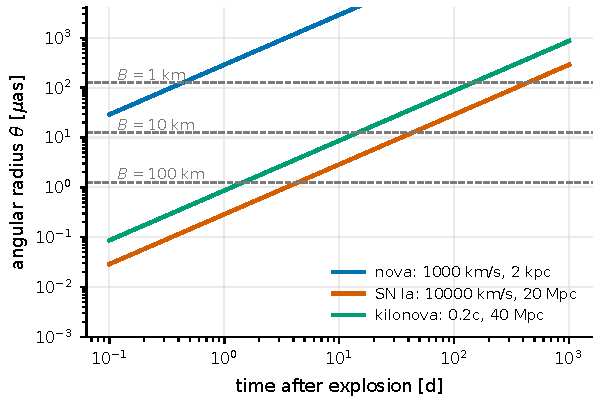
\includegraphics[width=0.92\linewidth]{figures/generated/chapter_13/ch13_expanding_fireball_resolution.pdf}
\caption{The angular radius of an expanding source is jointly determined by speed, time, and distance. A Galactic nova, though low in speed, wins by being nearby and enters the milliarcsecond regime fastest; low-redshift Type Ia supernovae and kilonovae are higher in speed but fall in the microarcsecond regime because they are too far away. The horizontal dashed lines are the \(\lambda/B\) resolution scales of different optical baselines at \(\lambda=0.5\,\mu\mathrm{m}\), they mark the threshold of ``who can be resolved by existing interferometers.''}
\label{fig:e20-expansion}
\end{figure}

Where does the \(v_{\rm exp}\) in Equation~\eqref{eq:e20-angular-expansion} come from? From spectral lines. A spectral line projects the line-of-sight velocity onto wavelength:
\begin{equation}
  v_{\rm los}\simeq c\,\frac{\lambda_{\rm obs}-\lambda_0}{\lambda_0},
  \label{eq:e20-doppler-line}
\end{equation}
\begin{formulaexplain}
\(v_{\rm los}\) is the line-of-sight velocity, \(\lambda_0\) is the laboratory wavelength, and \(\lambda_{\rm obs}\) is the observed wavelength. How far the line has shifted relative to its laboratory position ``imprints'' the velocity layer of the ejecta onto the wavelength axis.
\end{formulaexplain}
Here \(v_{\rm los}\) and \(c\) share the same units (\(\mathrm{cm\,s^{-1}}\)), and \(\lambda\) is the wavelength (cm or \(\text{\AA}\)). One must be careful: the blue edge of a P-Cygni absorption often represents the \textbf{fastest, outermost} material, the absorption minimum is closer to the layer of maximum optical depth, and the half-width of an emission line mixes several effects: geometry, optical depth, and density distribution. If one could measure the angular scale in each spectral-line channel, the data would become a set of \(\theta(v_{\rm los})\), which can distinguish a spherical shell, a bicone, an equatorial ring, or a polar wind.

How does one ``measure'' the angular scale? In intensity interferometry, the second-order correlation of a circularly symmetric uniform disk gives the squared visibility amplitude \(|V|^2\), whose first-order visibility modulus is the familiar Airy form (Chapter~\ref{chap:e11}):
\begin{equation}
  |V(B)|=
  \left|
  \frac{2J_1(\pi B\Theta/\lambda)}{\pi B\Theta/\lambda}
  \right|,
  \label{eq:e20-uniform-disk-visibility}
\end{equation}
\begin{formulaexplain}
\(|V(B)|\) is the visibility modulus of a uniform disk, \(\Theta=2\theta\) is the angular diameter, \(B\) is the projected baseline, \(\lambda\) is the wavelength, and \(J_1\) is the first-order Bessel function. The longer the baseline and the larger the source, the faster the visibility drops: this is precisely the quantitative meaning of ``resolving.''
\end{formulaexplain}
In this expression \(J_1\) is the first-order Bessel function (this is the standard result for circular-aperture diffraction, with its first zero at argument \(3.83\)), \(\Theta\) is the angular diameter (rad), \(B\) is the baseline (cm), and \(\lambda\) is the wavelength (cm). It assumes circular symmetry, a single wavelength, and no strong limb darkening; real novae and supernovae often require thin-shell, ring, ellipsoidal, or multi-component models. Combining the angular-expansion Equation~\eqref{eq:e20-angular-expansion} with the spectral-line velocity Equation~\eqref{eq:e20-doppler-line} yields a cosmic ruler independent of standard candles, the \textbf{expansion parallax}:
\begin{equation}
  D=\frac{v_{\rm exp}(t-t_0)}{\theta(t)}.
  \label{eq:e20-expansion-parallax}
\end{equation}
\begin{formulaexplain}
\(D\) is the geometric distance: the linear velocity times the time gives the linear radius, divided by the measured angular radius \(\theta(t)\) gives the distance. Its prerequisite is that \(v_{\rm exp}\) and \(\theta\) must correspond to the \textbf{same material layer}.
\end{formulaexplain}
This is a simple inversion of Equation~\eqref{eq:e20-angular-expansion}, but that prerequisite is where all the risk lies: if the spectral line measures the fast absorption of the outer layer while the angular scale comes from the continuum photosphere (which is more interior and slower), you are comparing two different velocity layers, and the distance will be systematically biased. A classical nova is itself a thermonuclear explosion on the surface of a white dwarf, with ejected mass \(10^{-5}\text{--}10^{-4}M_\odot\) and speeds exceeding \(10^3\,\mathrm{km\,s^{-1}}\); ever since Fermi discovered that novae are GeV \(\gamma\)-ray sources, the physical picture has been rewritten into a two-flow structure: a slow, dense equatorial ejection shaped by the binary orbit, struck by a fast polar wind that accelerates particles in the internal shock. The \(\gamma\)-ray emission of V959\,Mon lasted about \(12\,\mathrm{d}\), and high-resolution radio imaging showed the shock located exactly at the interface between the polar flow and the equatorial material, with a thermal ejecta mass of about \(4\times10^{-5}M_\odot\), in such a source \(v_{\rm exp}\) inherently contains two velocity components, and the spectral lines, radio images, and photon event table must be fit jointly \citep{2014Natur.514..339C,2014Sci...345..554A}.

Type Ia supernovae take another road: first they are calibrated into standard candles using the light-curve width. The Phillips relation corrects the peak absolute magnitude using the \(B\)-band decline rate \(\Delta m_{15}(B)\), and cosmological applications then write the corrected distance modulus as
\begin{equation}
  \mu = m_B - M_B + \alpha x_1-\beta C+\Delta_{\rm host},
  \label{eq:e20-snia-distance-modulus}
\end{equation}
\begin{formulaexplain}
\(\mu\) is the distance modulus, \(m_B,M_B\) are the observed and standardized peak magnitudes, \(x_1\) is the light-curve width, \(C\) is the color, and \(\alpha,\beta,\Delta_{\rm host}\) are fit from the sample. Standardizing a Type Ia is essentially correcting the luminosity a little at a time.
\end{formulaexplain}
Here \(m_B,M_B\) are magnitudes (dimensionless), \(x_1,C\) are dimensionless, and \(\Delta_{\rm host}\) is a host-galaxy-related correction term. A nearby Type Ia sample with \(m_B\sim10\text{--}16\) can yield high signal-to-noise light curves with a small telescope, while cosmological samples are often at \(m_B\sim22\text{--}25\). If one day one could \textbf{simultaneously} measure the angular expansion, one could use the geometric distance of Equation~\eqref{eq:e20-expansion-parallax} to cross-check this luminosity distance, which is very hard, because the ten-day Type Ia angular diameter is only of order microarcseconds, making it, in long-baseline optical intensity interferometry, a target of ``extreme difficulty but clear payoff'' \citep{1993ApJ...413L.105P,1998AJ....116.1009R,1999ApJ...517..565P}.

Is the ejecta round or not? Look at the polarization. The normalized Stokes parameters give the degree of linear polarization:
\begin{equation}
  q=\frac{Q}{I},\qquad
  u=\frac{U}{I},\qquad
  P=\sqrt{q^2+u^2},
  \label{eq:e20-stokes-polarization}
\end{equation}
\begin{formulaexplain}
\(q,u\) are the Stokes parameters normalized by the total intensity \(I\), and \(P\) is the degree of linear polarization. If the ejecta is perfectly spherically symmetric, the scattering cancels in all directions and \(P\to0\); once \(P\neq0\) appears, it signals a non-spherically-symmetric geometry.
\end{formulaexplain}
\(q,u,P\) are all dimensionless, usually reported as percentages. SN\,1999by near maximum had \(P\simeq0.3\text{--}0.8\%\), with an additional polarization variation of about \(0.4\%\) near Si\,II\,\(6150\,\text{\AA}\); models point to an overall asphericity of about \(20\%\), with the silicon layer and the continuum sharing broadly the same symmetry axis \citep{2001ApJ...556..302H}. So \(\theta(t)\) (from the photosphere shape), \(v_{\rm exp}\) (from the velocity layers), and \(P(t,\lambda)\) (from the scattering geometry) should all be interpreted within the same geometric model. This is precisely how ``keeping the frequency and polarization labels'' pays off for this class of source.

Finally there is the earliest, fastest window of a supernova, the \textbf{shock breakout}. When the shock is still at some depth \(d\) below the surface, radiation diffuses out first and forms a precursor. Let the local density be \(\rho\), the \textbf{opacity} \(\kappa\) (in units \(\mathrm{cm^2\,g^{-1}}\), about \(0.2\text{--}0.4\) for electron scattering, reaching order ten when heavy elements are present), so that the optical depth is \(\tau\simeq\kappa\rho d\). Breakout occurs at the moment when ``radiation diffusion finally catches up with the dynamical time'':
\begin{equation}
  t_{\rm diff}\simeq \frac{\tau d}{c}\simeq \frac{d}{v_s},
  \qquad
  \tau\simeq \frac{c}{v_s},
  \label{eq:e20-shock-breakout-condition}
\end{equation}
\begin{formulaexplain}
\(t_{\rm diff}\) is the time for photons to diffuse out of depth \(d\), and \(v_s\) is the shock velocity. A photon in a medium of optical depth \(\tau\) takes \(\tau\) random steps, so the diffusion time is about \(\tau d/c\); when this equals the time \(d/v_s\) for the shock to cross \(d\), the radiation ``leaks'' out, giving the breakout criterion \(\tau\simeq c/v_s\).
\end{formulaexplain}
Setting the two timescales equal gives the right-hand expression with no skipped logic: \(\tau d/c = d/v_s\Rightarrow\tau=c/v_s\). For a red supergiant \(v_s\sim1\text{--}2\times10^9\,\mathrm{cm\,s^{-1}}\), so \(\tau=c/v_s\sim15\text{--}30\), and the early energy appears mainly in the extreme ultraviolet or soft X-rays, with the optical discovery often lagging by several days. The GALEX ultraviolet data of SNLS-04D2dc caught the precursor before the shock reached the surface, constraining the envelope structure and the progenitor radius \citep{2008Sci...321..223S,2011ApJ...727..104C}. Such an hour-scale early signal pushes the pressure straight back onto the trigger system: the total delay from alarm, slewing, and target confirmation to the first exposure must be shorter than the signal's evolution, which is precisely what the end of this chapter will quantify.

\section{Kilonovae: turning multi-messenger delays into physical constraints}
\label{sec:e20-kilonova}

The 2017 event GW170817 gave transient astronomy a textbook timeline. Gravitational waves fixed the time and distance of the binary neutron star merger; Fermi/GBM and INTEGRAL saw GRB\,170817A about \(1.74\pm0.05\,\mathrm{s}\) later; within about ten-odd hours the optical counterpart was localized; and subsequently the UV/optical/near-infrared color swung rapidly from blue to red \citep{2017PhRvL.119p1101A,2017ApJ...848L..13A,2017ApJ...848L..12A,2017ApJ...848L..17C,2017Natur.551...75S}. What stitches these several messengers into a single event is precisely \textbf{time}.

The definition of a multi-messenger delay is so plain it is almost tautological:
\begin{equation}
  \Delta t_{a-b}=t_a-t_b .
  \label{eq:e20-mm-delay}
\end{equation}
\begin{formulaexplain}
\(\Delta t_{a-b}\) is the arrival-time difference between two messengers (or two bands). It is meaningful only under one prerequisite: \(t_a\) and \(t_b\) must be measured in the \textbf{same time-standard system}.
\end{formulaexplain}
This prerequisite is precisely the value of the unified clock of Chapter~\ref{chap:e13}: if the local clocks of different telescopes and different messengers are not first reduced to the same time standard, the \(1.74\,\mathrm{s}\) obtained by subtraction has no physical meaning whatsoever. And once the time standard is unified, interpreting this \(\Delta t\) must in turn be broken into three pieces, never swallowed whole:
\begin{equation}
  \Delta t_{\rm obs}
  =
  \Delta t_{\rm engine}
  +
  \Delta t_{\rm prop}
  +
  \Delta t_{\rm clock}.
  \label{eq:e20-delay-budget}
\end{equation}
\begin{formulaexplain}
The observed delay \(\Delta t_{\rm obs}\) = the intra-source emission delay \(\Delta t_{\rm engine}\) (how long from merger to jet breakout) + the propagation delay \(\Delta t_{\rm prop}\) (how fast or slow it travels en route) + the clock/processing error \(\Delta t_{\rm clock}\). Confuse the three, and you will mistake the physics of the source for a new propagation effect.
\end{formulaexplain}
Only after subtracting \(\Delta t_{\rm engine}\) and \(\Delta t_{\rm clock}\) clean can the remaining \(\Delta t_{\rm prop}\) be used to constrain fundamental questions such as ``whether gravitational waves and light travel at the same speed.'' If the source distance \(D\) is known, the order of magnitude of the permitted propagation-speed difference is
\begin{equation}
  \frac{|\Delta v|}{c}
  \lesssim
  \frac{|\Delta t_{\rm prop}|}{D/c}
  =
  2.4\times10^{-16}
  \left(\frac{\Delta t_{\rm prop}}{1\,{\rm s}}\right)
  \left(\frac{D}{40\,{\rm Mpc}}\right)^{-1}.
  \label{eq:e20-speed-difference}
\end{equation}
\begin{formulaexplain}
\(|\Delta v|/c\) is the order of magnitude of the relative speed difference between the two messengers, and \(D/c\) is the light travel time. The farther the distance, the longer the light travel time, and the same one-second propagation delay corresponds to a smaller speed difference, distant sources become an extremely sensitive ``speed balance.''
\end{formulaexplain}
Let us verify the coefficient: \(D=40\,\mathrm{Mpc}=1.234\times10^{26}\,\mathrm{cm}\), light travel time \(D/c=1.234\times10^{26}/3\times10^{10}=4.11\times10^{15}\,\mathrm{s}\), so \(1\,\mathrm{s}/(D/c)=2.4\times10^{-16}\). The \textbf{usage} of this formula must be handled with care: one must never stuff the entire \(1.74\,\mathrm{s}\) into it as a propagation delay, because the GRB emission itself may be later than the merger (that belongs to \(\Delta t_{\rm engine}\)). Its true role is to lock ``any unknown new propagation effect'' into the cage of order \(\sim10^{-16}\).

\begin{figure}[tbp]
\centering
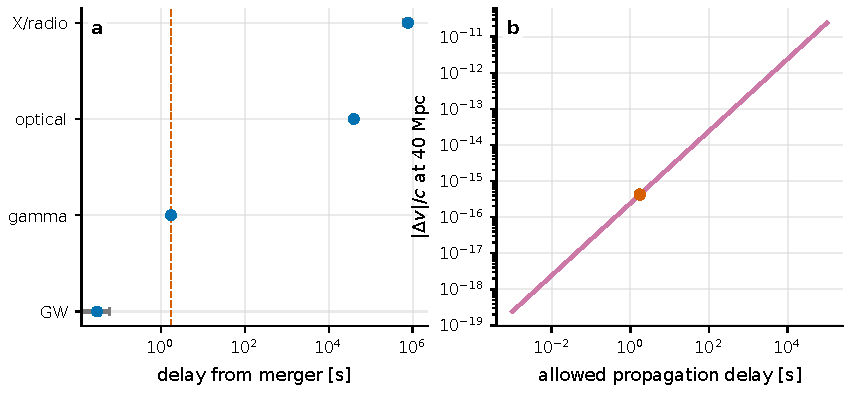
\includegraphics[width=0.92\linewidth]{figures/generated/chapter_13/ch13_multimessenger_delay.pdf}
\caption{Two readings of a multi-messenger delay. The left panel compares the arrival times of the channels after merger: gravitational waves and \(\gamma\)-rays on the second scale, the optical counterpart limited by localization and the day-night cycle and often on the hour scale, and X-rays/radio emerging on day-to-month scales. The right panel converts the propagation delay into the order of magnitude of \(|\Delta v|/c\) at \(40\,\mathrm{Mpc}\), the more uncertain the intra-source emission delay, the more conservative the propagation constraint one can give.}
\label{fig:e20-mm-delay}
\end{figure}

Where does the light of a kilonova come from? From the thermalization of the \(r\)-process (\(r\)-process) radioactive decay in the neutron-rich ejecta. A commonly used scaling is
\begin{equation}
  \dot q(t)\simeq
  2\times10^{10}
  \left(\frac{t}{1\,{\rm d}}\right)^{-1.3}
  {\rm erg\,s^{-1}\,g^{-1}},
  \label{eq:e20-rprocess-heating}
\end{equation}
\begin{formulaexplain}
\(\dot q(t)\) is the heating rate per unit mass of the \(r\)-process material, decaying with time approximately as \(t^{-1.3}\). The power source of a kilonova is not residual heat, not recombination, but this line of radioactive decay.
\end{formulaexplain}
\(\dot q\) is in units of \(\mathrm{erg\,s^{-1}\,g^{-1}}\). What actually enters the luminosity is \(\epsilon_{\rm th}M_{\rm ej}\dot q\), where the thermalization efficiency \(\epsilon_{\rm th}<1\) and \(M_{\rm ej}\) is the ejecta mass. When the light curve peaks is set by the \textbf{diffusion timescale}: the photons must diffuse out from the interior of the ejecta, and the thicker, slower, and more opaque the ejecta, the later they emerge:
\begin{equation}
  t_{\rm pk}\simeq
  \left(\frac{\kappa M_{\rm ej}}{4\pi v_{\rm ej}c}\right)^{1/2}
  =
  0.6\,{\rm d}
  \left(\frac{\kappa}{0.5\,{\rm cm^2\,g^{-1}}}\right)^{1/2}
  \left(\frac{M_{\rm ej}}{0.01M_\odot}\right)^{1/2}
  \left(\frac{v_{\rm ej}}{0.3c}\right)^{-1/2}.
  \label{eq:e20-kilonova-diffusion}
\end{equation}
\begin{formulaexplain}
\(t_{\rm pk}\) is the kilonova peak time, \(\kappa\) is the opacity, \(M_{\rm ej}\) is the ejecta mass, and \(v_{\rm ej}\) is the velocity. The larger the opacity, the larger the mass, and the lower the velocity, the later the peak and the redder the color.
\end{formulaexplain}
Let us verify the \(0.6\,\mathrm{d}\) coefficient: \(\kappa=0.5\,\mathrm{cm^2\,g^{-1}}\), \(M_{\rm ej}=0.01M_\odot=1.99\times10^{31}\,\mathrm{g}\), \(v_{\rm ej}=0.3c=9\times10^9\,\mathrm{cm\,s^{-1}}\), \(c=3\times10^{10}\,\mathrm{cm\,s^{-1}}\). The numerator \(\kappa M_{\rm ej}=9.95\times10^{30}\), the denominator \(4\pi v_{\rm ej}c=4\pi\times9\times10^9\times3\times10^{10}=3.39\times10^{21}\), the ratio \(2.93\times10^{9}\,\mathrm{s^2}\), and taking the square root gives \(5.4\times10^4\,\mathrm{s}\approx0.63\,\mathrm{d}\). The orders of magnitude are then clear: lanthanide-poor ejecta have \(\kappa\sim0.3\text{--}1\,\mathrm{cm^2\,g^{-1}}\), peaking around one day and blueward; lanthanide-rich ejecta have \(\kappa\sim5\text{--}30\,\mathrm{cm^2\,g^{-1}}\), pushing the peak to several days or even ten days and turning toward the near-infrared.

The early spectrum can be approximated by a blackbody, translating the color evolution in one step into radius and temperature:
\begin{equation}
  L_{\rm bol}=4\pi R_{\rm BB}^2\sigma_{\rm SB}T_{\rm BB}^4 .
  \label{eq:e20-kilonova-blackbody}
\end{equation}
\begin{formulaexplain}
\(L_{\rm bol}\) is the total radiative luminosity, \(R_{\rm BB},T_{\rm BB}\) are the blackbody radius and temperature, and \(\sigma_{\rm SB}\) is the Stefan--Boltzmann constant. Given the SED, fitting out \(R_{\rm BB},T_{\rm BB}\) translates ``color changing with time'' into ``the emitting surface is expanding and cooling.''
\end{formulaexplain}
GW170817 at about \(0.6\,\mathrm{d}\) can be described by \(T_{\rm BB}\simeq8300\,\mathrm{K}\), \(R_{\rm BB}\simeq4.5\times10^{14}\,\mathrm{cm}\), \(L_{\rm bol}\simeq5\times10^{41}\,\mathrm{erg\,s^{-1}}\), corresponding to \(v\simeq0.3c\). Subsequently the SED rapidly departed from a single blackbody: the ultraviolet/blue faded while the near-infrared relatively strengthened. This forces at least a two-component model: a blue component with \(M_{\rm ej}\sim0.01M_\odot\), \(v\sim0.27\text{--}0.3c\), and a red component with \(M_{\rm ej}\sim0.04M_\odot\), \(v\sim0.1c\); a three-component model further singles out an intermediate-opacity ``purple component'' \citep{2017Natur.551...75S,2017ApJ...848L..17C,2017ApJ...848L..27T,2017Sci...358.1565E}. A single component cannot explain ``early blue, late red'', which is itself the data telling us that the ejecta has structure.

\begin{figure}[tbp]
\centering
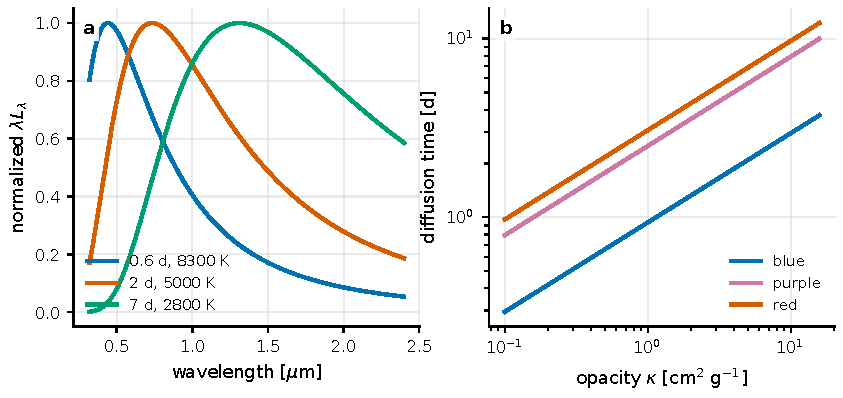
\includegraphics[width=0.92\linewidth]{figures/generated/chapter_13/ch13_kilonova_color_evolution.pdf}
\caption{The blue-to-red evolution of a kilonova. The left panel uses three blackbody SEDs to show the peak wavelength shifting to the infrared as the temperature drops (Wien shift); the right panel uses the diffusion-timescale Equation~\eqref{eq:e20-kilonova-diffusion} to show that the larger the opacity, the larger the mass, and the lower the velocity, the later the peak. GW170817's blue component is fast and low-opacity while its red component is slow and high-opacity, so a single ejecta component cannot simultaneously explain the early blue light and the late near-infrared.}
\label{fig:e20-kilonova}
\end{figure}

Gravitational waves also throw in a bonus treasure, the \textbf{standard siren}: the amplitude of the merger waveform directly gives the luminosity distance, without needing the distance ladder. At low redshift it can be roughly written as
\begin{equation}
  H_0\simeq \frac{cz_{\rm host}}{D_L},
  \label{eq:e20-standard-siren}
\end{equation}
\begin{formulaexplain}
\(H_0\) is the Hubble constant, \(z_{\rm host}\) is the host-galaxy redshift, and \(D_L\) is the luminosity distance given by the gravitational waves. The redshift (recession velocity) divided by the distance is the expansion rate, only here the distance comes from gravitational waves, not from candles.
\end{formulaexplain}
\(z_{\rm host}\) is dimensionless, \(D_L\) is in cm or Mpc, and \(H_0\) is in \(\mathrm{km\,s^{-1}\,Mpc^{-1}}\). The main degeneracy of GW170817 comes from inclination and distance: a binary pointing straight at us is both brighter and harder to constrain in inclination. The electromagnetic counterpart rendered great service here: it gave the host, the redshift, the jet viewing angle, and the ejecta geometry, breaking part of the degeneracy for the gravitational waves. This is the essence of multi-messenger astronomy: a single physical event is projected by gravitational waves, \(\gamma\)-rays, and the optical each onto one facet, and then a joint likelihood stitches them back into a three-dimensional truth.

\section{Gamma-ray burst afterglows: writing the jet geometry into the light-curve slopes}
\label{sec:e20-grb}

The prompt emission of a gamma-ray burst gives the high-energy trigger, but the \textbf{afterglow} is the external-shock physics that can be slowly tracked. After a relativistic thin shell plows into the external medium, the relation between the observed time \(t\) and the shock radius \(R\) and Lorentz factor \(\Gamma\) is approximately
\begin{equation}
  t\simeq \frac{(1+z)R}{4\Gamma^2c}.
  \label{eq:e20-grb-arrival-time}
\end{equation}
\begin{formulaexplain}
\(t\) is the observed arrival time, \(R\) is the shock radius, \(\Gamma\) is the Lorentz factor, and \(z\) is the redshift. The factor \(1/\Gamma^2\) is the combined result of relativistic beaming and the light travel time effect: the source moves almost as fast as the light it emits, compressing a very large \(R\) into an extremely short observed time.
\end{formulaexplain}
The astonishing thing about this formula is that \(\Gamma^2\): a typical early afterglow has \(\Gamma\sim10\text{--}300\), \(R\sim10^{16}\text{--}10^{18}\,\mathrm{cm}\), yet the optical signal can enter the telescope's field of view within tens of seconds to a few minutes after the trigger, an astronomical-scale radius compressed into an observation so fast that only a robotic telescope can chase it \citep{1997ApJ...476..232M,1998ApJ...497L..17S,1998Natur.395..670G,1999PhR...314..575P,2004RvMP...76.1143P,2006ARA&A..44..507W}.

The afterglow light comes from synchrotron radiation by shock-accelerated electrons. Let the electron energy spectrum be a power law:
\begin{equation}
  N(\gamma_e)\,d\gamma_e \propto \gamma_e^{-p}\,d\gamma_e,
  \qquad \gamma_e>\gamma_m,
  \label{eq:e20-electron-powerlaw}
\end{equation}
\begin{formulaexplain}
\(N(\gamma_e)\) is the distribution of the electron Lorentz factor, \(p\) is the energy-spectrum index (typically \(2\text{--}2.5\)), and \(\gamma_m\) is the low-energy cutoff. The slope of the synchrotron afterglow spectrum is ultimately governed by this single number \(p\).
\end{formulaexplain}
Observationally, one usually first compresses the light curve and color into two slopes: the temporal decay index \(\alpha\) and the spectral index \(\beta\):
\begin{equation}
  F_\nu(t)\propto t^{-\alpha}\nu^{-\beta}.
  \label{eq:e20-afterglow-powerlaw}
\end{equation}
\begin{formulaexplain}
\(F_\nu(t)\) is the afterglow flux density, \(\alpha\) governs ``how it dims with time,'' and \(\beta\) governs ``how the spectrum tilts with frequency.'' The two slopes are the afterglow's most compact fingerprint.
\end{formulaexplain}
In a uniform medium, adiabatic, slow-cooling case with the observing frequency in the interval \(\nu_m<\nu<\nu_c\), these two slopes are not independent but are locked together by the same \(p\):
\begin{equation}
  \beta=\frac{p-1}{2},
  \qquad
  \alpha=\frac{3(p-1)}{4}.
  \label{eq:e20-closure-relation}
\end{equation}
\begin{formulaexplain}
This is a \textbf{closure relation}: it binds the observed \(\alpha,\beta\) to the electron index \(p\). If the data clearly deviate from it, then at least one of the assumptions ``simple medium / weak energy injection / non-evolving microphysics'' has collapsed.
\end{formulaexplain}
Dividing the two immediately reveals the structure: \(\alpha/\beta=3/2\), a fixed value independent of \(p\), a hard prediction of this interval. Substituting \(p=2.2\) gives \(\beta\simeq0.6\), \(\alpha\simeq0.9\); if the observing frequency moves to \(\nu>\nu_c\) (the fast-cooling segment), it becomes \(\alpha=(3p-2)/4\). Observationally, an afterglow one day after the burst is often at magnitude \(19\text{--}20\), with polarization reaching a few percent to about \(10\%\), directly related to synchrotron radiation and jet geometry \citep{2004RvMP...76.1143P,2006ARA&A..44..507W}.

\begin{figure}[tbp]
\centering
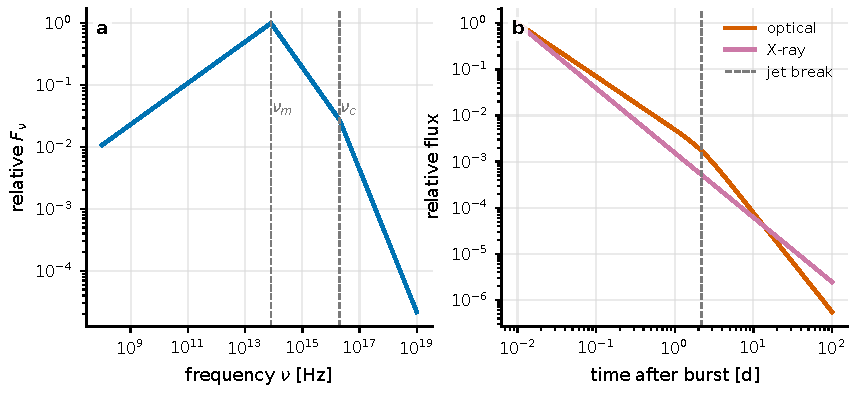
\includegraphics[width=0.92\linewidth]{figures/generated/chapter_13/ch13_afterglow_synchrotron_breaks.pdf}
\caption{The synchrotron reading of a gamma-ray burst afterglow. The left panel shows the characteristic frequencies \(\nu_m\) (minimum electron) and \(\nu_c\) (cooling) slicing the spectrum into intervals of different slope; the right panel shows the light curve steepening across the jet break. If the optical and X-ray are not in the same spectral segment, their \(\alpha,\beta\) need not be the same. One must first judge the position of the observing frequency relative to \(\nu_m,\nu_c\) before applying the closure relation.}
\label{fig:e20-afterglow}
\end{figure}

A jet is not isotropic. When \(\Gamma\) decays to about \(1/\theta_j\), the observer for the first time ``sees the edge of the jet,'' and the light curve exhibits an \textbf{achromatic jet break}. A commonly used estimate is
\begin{equation}
  \theta_j\simeq
  0.10
  \left(\frac{t_j}{1\,{\rm d}}\right)^{3/8}
  \left(\frac{1+z}{2}\right)^{-3/8}
  \left(\frac{E_{\rm iso,52}}{n_0}\right)^{-1/8},
  \label{eq:e20-jet-opening-angle}
\end{equation}
\begin{formulaexplain}
\(\theta_j\) is the jet half-opening angle (rad), \(t_j\) is the jet break time, \(E_{\rm iso,52}\) is the isotropic energy in units of \(10^{52}\,\mathrm{erg}\), and \(n_0\) is the external number density (\(\mathrm{cm^{-3}}\)). The later the break, the wider the jet typically is.
\end{formulaexplain}
Notice those \textbf{very weak} exponents: \(3/8\) and \(1/8\). They are good news for error propagation: even if \(E_{\rm iso}\) or \(n\) each has an order-of-magnitude uncertainty, a factor of \(10\) change in \((E_{\rm iso}/n)\), passed through the \(1/8\) power, changes \(\theta_j\) by only about \(10^{1/8}\approx1.33\) times, i.e.\ thirty percent. The real risk lies not in these parameters but in \textbf{misclassification}: a color-change break, energy injection, a density jump, or even a superimposed supernova bump can all be mistaken for a jet break \citep{2003Natur.423..847H,2004ApJ...611.1005G}. GRB\,980425/SN\,1998bw and GRB\,030329/SN\,2003dh linked long bursts with broad-lined Type Ic supernovae, while the link between short bursts and binary neutron star mergers became multi-messenger ironclad proof after GW170817. Gamma-ray bursts force a telescope system to simultaneously handle a second-scale high-energy trigger, a minute-scale optical flash, an hour-to-day afterglow, and a week-to-month radio calorimetry, and the event table must, besides the flux, keep the time reference and band matching for each stage.

\section{Tidal disruption events: reading the black hole mass from the fallback rate}
\label{sec:e20-tde}

When a star comes too close to a supermassive black hole, it is torn apart, a \textbf{tidal disruption event} (TDE). The tearing occurs inside the tidal radius:
\begin{equation}
  r_t\simeq R_\ast\left(\frac{M_\bullet}{M_\ast}\right)^{1/3},
  \label{eq:e20-tidal-radius}
\end{equation}
\begin{formulaexplain}
\(r_t\) is the tidal radius, \(M_\bullet\) is the black hole mass, and \(M_\ast,R_\ast\) are the stellar mass and radius. Once the star enters within \(r_t\), the gravitational difference of the black hole across its two ends exceeds its own self-gravity, stretching it into a noodle.
\end{formulaexplain}
\(r_t,R_\ast\) are in cm, and \(M_\bullet,M_\ast\) are in g. Whether a bright flare is produced also requires comparison with one more scale, the Schwarzschild radius:
\begin{equation}
  r_s=\frac{2GM_\bullet}{c^2}.
  \label{eq:e20-schwarzschild-radius-tde}
\end{equation}
\begin{formulaexplain}
\(r_s\) is the black hole's Schwarzschild radius. Compare \(r_t\) with \(r_s\): if \(r_t\lesssim r_s\), the star is swallowed whole before it can be torn apart, and no bright flare is seen.
\end{formulaexplain}
Note that \(r_t\propto M_\bullet^{1/3}\) while \(r_s\propto M_\bullet\); the heavier the black hole, the faster \(r_s\) catches up. So main-sequence-star TDEs are most common for \(M_\bullet\sim10^5\text{--}10^7M_\odot\), and around \(10^8M_\odot\), \(r_s\) approaches or even exceeds \(r_t\), and the selection effect grows stronger \citep{1988Natur.333..523R,2021ARA&A..59...21G}.

After being torn apart, half the debris is bound and half escapes. The bound debris that returns to pericenter earliest gives the \textbf{fallback timescale}:
\begin{equation}
  t_{\rm min}\simeq
  41\,{\rm d}
  \left(\frac{M_\bullet}{10^6M_\odot}\right)^{1/2}
  \left(\frac{M_\ast}{M_\odot}\right)^{-1}
  \left(\frac{R_\ast}{R_\odot}\right)^{3/2}.
  \label{eq:e20-tde-fallback-time}
\end{equation}
\begin{formulaexplain}
\(t_{\rm min}\) is the time for the most-bound debris to orbit back to pericenter, given by the Keplerian period of the most-bound orbit, hence growing as \(M_\bullet^{1/2}\). It is the yardstick of the TDE rise timescale.
\end{formulaexplain}
The heavier the black hole, the longer \(t_{\rm min}\) (\(\propto M_\bullet^{1/2}\)), so the rise time itself hides the black hole mass. The fallback rate then transitions into the classic \(t^{-5/3}\) decay:
\begin{equation}
  \dot M_{\rm fb}\simeq
  \frac{M_\ast}{3t_{\rm min}}
  \left(\frac{t}{t_{\rm min}}\right)^{-5/3}.
  \label{eq:e20-tde-fallback-rate}
\end{equation}
\begin{formulaexplain}
\(\dot M_{\rm fb}\) is the debris fallback rate. The ideal \(t^{-5/3}\) decay comes from the uniform distribution of debris energy and is the classic fingerprint of a TDE; but the observed luminosity is also smoothed by circularization (the process by which debris orbits collide, dissipate, and wind into an accretion disk) and reprocessing, and need not follow it strictly.
\end{formulaexplain}
\(\dot M_{\rm fb}\) is commonly in \(M_\odot\,\mathrm{yr^{-1}}\). How fierce is this fallback? Compare it with the Eddington accretion rate:
\begin{equation}
  \dot M_{\rm Edd}
  =
  \frac{L_{\rm Edd}}{\eta c^2}
  \simeq
  0.022
  \left(\frac{M_\bullet}{10^6M_\odot}\right)
  \left(\frac{\eta}{0.1}\right)^{-1}
  M_\odot\,{\rm yr^{-1}} ,
  \label{eq:e20-eddington-rate}
\end{equation}
\begin{formulaexplain}
\(\dot M_{\rm Edd}\) is the Eddington accretion rate, and \(\eta\) is the radiative efficiency. Comparing \(\dot M_{\rm fb}\) with it tells you whether the fallback has surged into a super-Eddington phase.
\end{formulaexplain}
Let us verify the \(0.022\): \(L_{\rm Edd}=1.26\times10^{38}(M_\bullet/M_\odot)\,\mathrm{erg\,s^{-1}}=1.26\times10^{44}\,\mathrm{erg\,s^{-1}}\) (for \(10^6M_\odot\)), \(\eta c^2=0.1\times(3\times10^{10})^2=9\times10^{19}\), so \(\dot M_{\rm Edd}=1.4\times10^{24}\,\mathrm{g\,s^{-1}}\); converting to \(M_\odot\,\mathrm{yr^{-1}}\) (multiply by \(3.156\times10^7\,\mathrm{s\,yr^{-1}}\), divide by \(1.989\times10^{33}\,\mathrm{g}\)) gives \(0.022\). For a \(10^6M_\odot\) black hole, the peak fallback rate of a solar-type star can significantly exceed Eddington, but the \textbf{optical} luminosity need not exceed it likewise, because circularization, stellar winds, obscuration, and reprocessing move the inner-disk energy into the UV/optical and redistribute it.

\begin{figure}[tbp]
\centering
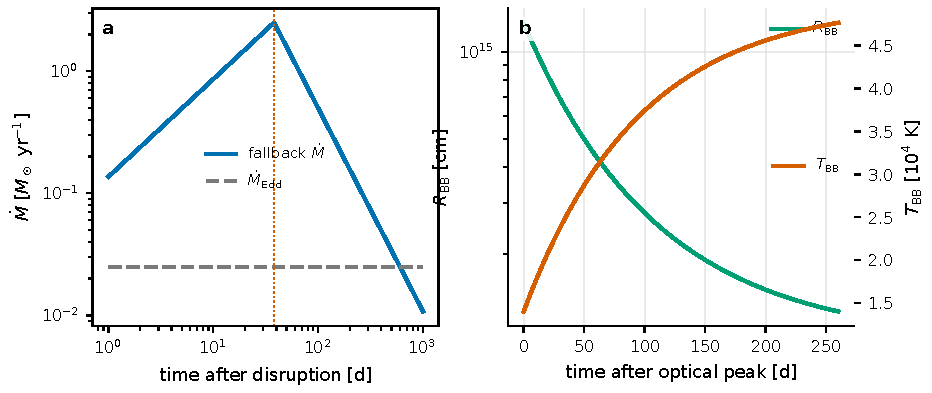
\includegraphics[width=0.92\linewidth]{figures/generated/chapter_13/ch13_tde_fallback_reprocessing.pdf}
\caption{TDE fallback and reprocessing. The left panel shows the \(t^{-5/3}\) fallback entering the decay segment on the scale of tens of days, remaining for a long time above the Eddington accretion rate of a \(10^6M_\odot\) black hole; the right panel gives a typical evolution of the optical/UV blackbody photosphere: the radius contracts from order \(10^{15}\,\mathrm{cm}\) to \(10^{14}\,\mathrm{cm}\), and the temperature rises from order \(10^4\,\mathrm{K}\) to several \(10^4\,\mathrm{K}\).}
\label{fig:e20-tde}
\end{figure}

The blackbody radius of an optical TDE is typically \(10^{14}\text{--}10^{15}\,\mathrm{cm}\), much larger than a few times the \(r_s\) of a \(10^6M_\odot\) black hole; the temperature is often a few \(\times10^4\,\mathrm{K}\), and the evolution is slower than an ordinary supernova. AT2018zr was the first TDE in the early ZTF sample to capture the full rise, with the earliest detection about \(50\,\mathrm{d}\) before peak; its blackbody temperature was about \(1.4\times10^4\,\mathrm{K}\) early on and rose to \(>5\times10^4\,\mathrm{K}\) later, the radius fell from \(10^{15.1}\,\mathrm{cm}\) to \(<10^{14}\,\mathrm{cm}\), and the X-ray luminosity was several orders of magnitude below the contemporaneous optical/UV blackbody, indicating that obscuration or reprocessing cannot be neglected \citep{2019ApJ...872..198V,2021ARA&A..59...21G}. Jetted TDEs (such as Swift\,J1644+57) push the event table toward high energies and rapid variability: the X-rays flicker violently, and the radio tracks the interaction of the outflow with the medium \citep{2011Sci...333..203B}. As for the possible association of TDEs with high-energy neutrinos, that is yet another class of multi-messenger problem requiring a triple coincidence in time, direction, and energy to judge \citep{2021NatAs...5..510S}. Even in such a ``slow'' transient, the event table must still retain complete time information: judging whether a high-energy event belongs to a given optical flare relies on whether the celestial position, time delay, energy, direction error, and source evolution are mutually consistent.

\section{Target-of-opportunity observation: computing ``fast'' and ``error'' together}
\label{sec:e20-tooo}

The success or failure of transient observation is often decided by response speed. But ``fast'' must be quantified, otherwise it is only a slogan. A practical condition is that the total delay from trigger to the first effective exposure must be shorter than the evolution timescale of the source you wish to sample:
\begin{equation}
  t_{\rm alert}+t_{\rm slew}+t_{\rm acq}+t_{\rm exp}
  < f_{\rm samp}\,t_{\rm evol},
  \label{eq:e20-response-budget}
\end{equation}
\begin{formulaexplain}
The left side is the response budget: alert issuance \(t_{\rm alert}\) + telescope slewing \(t_{\rm slew}\) + target confirmation and guiding \(t_{\rm acq}\) + the first effective exposure \(t_{\rm exp}\); the right side is the source evolution timescale \(t_{\rm evol}\) you wish to sample, times a sampling factor \(f_{\rm samp}\). Target-of-opportunity observation is about satisfying this inequality.
\end{formulaexplain}
If you want to \textbf{resolve} the rise rather than just catch a single point, then \(f_{\rm samp}\sim0.1\) is reasonable (the sampling must be ten times faster than the evolution). Substituting the various source types of this chapter: the \(t_{\rm evol}\) of a GRB optical flash can be less than \(10^3\,\mathrm{s}\), the blue-light phase of a GW counterpart is about one day, the early radio/spectral structure of a nova changes within days to weeks, and the rise timescale of a TDE is often tens of days. The same formula turns ``how fast, exactly'' from an emotion into a checkable number.

Having secured the target, one must still compute whether the exposure is deep enough. The signal-to-noise ratio of ordinary imaging is
\begin{equation}
  {\rm SNR}=
  \frac{N_s}
  {\left(N_s+N_b+n_{\rm pix}\sigma_{\rm read}^2\right)^{1/2}},
  \label{eq:e20-imaging-snr}
\end{equation}
\begin{formulaexplain}
\({\rm SNR}\) is the imaging signal-to-noise ratio, \(N_s\) is the source count, \(N_b\) is the background count, and \(n_{\rm pix}\sigma_{\rm read}^2\) is the read noise summed over the pixels within the aperture. Those three terms in the denominator are precisely the sum of the three kinds of error: ``source's own fluctuation + background fluctuation + electronic noise.''
\end{formulaexplain}
\(N_s,N_b\) are counts (dimensionless), \(n_{\rm pix}\) is the number of pixels within the aperture, and \(\sigma_{\rm read}\) is the read noise per pixel (in electrons). When the source is bright (\(N_s\gg N_b,\,n_{\rm pix}\sigma_{\rm read}^2\)), the denominator tends to \(\sqrt{N_s}\), recovering the shot-noise limit \({\rm SNR}\to\sqrt{N_s}\) of Chapter~\ref{chap:e03}; when the source is faint, the background and read noise take over, which is precisely why deep-field transients are hard to do.

Finally, do not forget that \textbf{host association} is also a statistical judgment with errors, not ``it looks close so it must be a match.'' If the transient localization error radius is \(r\) and the surface density of background galaxies down to depth \(m\) is \(\Sigma(<m)\), then the \textbf{chance coincidence probability} of randomly hitting a background galaxy is
\begin{equation}
  P_{\rm cc}=1-\exp[-\pi r^2\Sigma(<m)].
  \label{eq:e20-chance-coincidence}
\end{equation}
\begin{formulaexplain}
\(P_{\rm cc}\) is the chance host-coincidence probability, \(r\) is the localization error radius, and \(\Sigma(<m)\) is the surface density of background galaxies. It is in fact a Poisson result: the probability that ``there is at least one background galaxy within the error circle'' is \(1-e^{-\langle N\rangle}\), with the expected number \(\langle N\rangle=\pi r^2\Sigma\).
\end{formulaexplain}
In this expression \(r\) is in rad or arcsec, \(\Sigma(<m)\) is the number of galaxies per unit solid angle (e.g.\ \(\mathrm{arcsec^{-2}}\)), and the product \(\pi r^2\Sigma\) is dimensionless. The worse the localization and the denser the galaxies, the larger \(P_{\rm cc}\) and the less trustworthy the host association. GW170817 relied on the addition of the Virgo detector to shrink the sky region from over a hundred to a few tens of square degrees, allowing the optical survey to lock down the host on the same night; TDEs, conversely, require sub-arcsecond astrometry to prove that the flare truly sits at the galactic nucleus. The same \(P_{\rm cc}\) governs everything from gravitational-wave localization to nuclear-transient confirmation \citep{2017PhRvL.119p1101A,2017ApJ...848L..12A,2019ApJ...872..198V}.

Listing the timescales, observables, and main risks of the six source classes of this chapter side by side, for easy comparison:
\begin{longtable}{@{}p{0.14\linewidth}p{0.18\linewidth}p{0.28\linewidth}p{0.28\linewidth}@{}}
\toprule
Source class & Key timescale & Typical observables & Main risk \\
\midrule
Classical nova & Days to months & Line velocity, radio angular scale, \(\gamma\)-ray window & Multiple velocity components bias the expansion parallax. \\
Type Ia supernova & Days to weeks & Light-curve width, color, Si\,II velocity, polarization, microarcsecond angular scale & Luminosity calibration and angular scale come from different physical layers. \\
Core-collapse & Minutes to days & UV/soft X-ray outburst, early spectrum, polarization & Triggering too late misses the progenitor-radius information. \\
Kilonova & Hours to ten days & GW distance, \(\gamma\)-ray delay, color and near-infrared evolution & Opacity, viewing angle, and ejecta geometry are mutually degenerate. \\
Gamma-ray burst & Seconds to months & \(\alpha,\beta\), jet break, polarization, radio calorimetry & A color-change break or energy injection misjudges the jet geometry. \\
Tidal disruption & Weeks to years & Rise timescale, nuclear position, \(T_{\rm BB}\), \(R_{\rm BB}\), X-ray/optical ratio & AGN-variable contamination and non-unique reprocessing geometry. \\
\bottomrule
\end{longtable}

\section*{Chapter Summary}
\addcontentsline{toc}{section}{Chapter Summary}

\begin{itemize}
  \item \textbf{The information of a transient is in time.} The light curve is a binned product that smears away the onset time and fine structure; the unbinned inhomogeneous Poisson likelihood Equation~\eqref{eq:e20-poisson-likelihood} eats the event times \(t_j\) directly, which is precisely why Chapter~\ref{chap:e13} insists on keeping the time/frequency/polarization label of every photon.
  \item \textbf{Triggering is inference, not an alarm.} Use the odds ratio Equation~\eqref{eq:e20-trigger-odds} to put ``prior rarity'' and ``data likelihood'' into the judgment together; false triggers are controlled by the Poisson-tail probability Equation~\eqref{eq:e20-false-alarm}, but the true number of false alarms must be multiplied by the trials factor over time windows, pixels, energy channels, and templates.
  \item \textbf{Transient sources are mostly thermal chaotic light.} The coherence time of a broadband blackbody photosphere is only a femtosecond (\(\tau_c\simeq1/\Delta\nu\)), and within a millisecond bin the counts degenerate into pure Poisson shot noise; to touch the coherence information one must rely on nanosecond/picosecond intensity interferometry, whose precision is set by the photon-pair number Equation~\eqref{eq:e20-pair-statistics}. Coherent emission such as FRBs and pulsars exposes itself through an extremely high brightness temperature.
  \item \textbf{Geometry links speed, time, and angular scale into a cosmic ruler.} The angular-expansion Equation~\eqref{eq:e20-angular-expansion} plus the spectral-line velocity Equation~\eqref{eq:e20-doppler-line} give the expansion parallax Equation~\eqref{eq:e20-expansion-parallax}, but the velocity and the angular scale must correspond to the same material layer, otherwise the distance is systematically biased.
  \item \textbf{Multi-messenger astronomy is stitched by time.} A delay is meaningful only under a unified time standard (Equation~\eqref{eq:e20-mm-delay}), and must be split into intra-source emission, propagation, and clock parts (Equation~\eqref{eq:e20-delay-budget}); great distance lets a second-scale delay correspond to a speed-difference constraint of \(\sim10^{-16}\) (Equation~\eqref{eq:e20-speed-difference}).
  \item \textbf{``Fast'' must be quantified, and the host must be verified.} The response budget Equation~\eqref{eq:e20-response-budget} turns speed into a checkable inequality; the chance-coincidence probability Equation~\eqref{eq:e20-chance-coincidence} reminds us that host association, like triggering, is a statistical judgment with errors. The error budget of Chapter~\ref{chap:e15} will fold all of these into the feasibility analysis.
\end{itemize}

\medskip
\noindent\textbf{Questions to Ponder}
\begin{itemize}
  \item A GRB trigger uses a window of \(\Delta t=0.05\,\mathrm{s}\) and a background rate \(b=2\,\mathrm{s^{-1}}\). If one night searches \(10^{9}\) independent windows, roughly what trigger threshold \(n\) should be chosen to keep the expected number of false alarms below 1? (Hint: use Equation~\eqref{eq:e20-false-alarm} to first compute the single-window \(P_{\rm FA}\), then multiply by the number of trials.)
  \item If the spectral line of a nova gives the outermost \(v_{\rm exp}=1.5\times10^8\,\mathrm{cm\,s^{-1}}\), while the angular scale actually comes from a more interior continuum photosphere with a velocity only \(0.7\) times as large, will the distance obtained from Equation~\eqref{eq:e20-expansion-parallax} be too large or too small, and by how much?
  \item Why, when doing photometry of a broadband thermal transient, can one safely use \(\sqrt N\) errors, whereas doing intensity interferometry one must return to the photon-pair number Equation~\eqref{eq:e20-pair-statistics}? At which time scale is each of the two ``looking at'' the signal?
\end{itemize}
